\documentclass{sigchi}

% pandoc setup %



\usepackage[backend=biber]{biblatex}
\addbibresource{references.bib}

\providecommand{\tightlist}{%
  \setlength{\itemsep}{0pt}\setlength{\parskip}{0pt}}

% end pandoc setup %

% Use this section to set the ACM copyright statement (e.g. for
% preprints).  Consult the conference website for the camera-ready
% copyright statement.

% Copyright
\CopyrightYear{2020}
%\setcopyright{acmcopyright}
\setcopyright{acmlicensed}
%\setcopyright{rightsretained}
%\setcopyright{usgov}
%\setcopyright{usgovmixed}
%\setcopyright{cagov}
%\setcopyright{cagovmixed}
% DOI
\doi{https://doi.org/10.1145/3313831.XXXXXXX}
% ISBN
\isbn{978-1-4503-6708-0/20/04}
%Conference
\conferenceinfo{CHI'20,}{April  25--30, 2020, Honolulu, HI, USA}
%Price
\acmPrice{\$15.00}

% Use this command to override the default ACM copyright statement
% (e.g. for preprints).  Consult the conference website for the
% camera-ready copyright statement.

%% HOW TO OVERRIDE THE DEFAULT COPYRIGHT STRIP --
%% Please note you need to make sure the copy for your specific
%% license is used here!
% \toappear{
% Permission to make digital or hard copies of all or part of this work
% for personal or classroom use is granted without fee provided that
% copies are not made or distributed for profit or commercial advantage
% and that copies bear this notice and the full citation on the first
% page. Copyrights for components of this work owned by others than ACM
% must be honored. Abstracting with credit is permitted. To copy
% otherwise, or republish, to post on servers or to redistribute to
% lists, requires prior specific permission and/or a fee. Request
% permissions from \href{mailto:Permissions@acm.org}{Permissions@acm.org}. \\
% \emph{CHI '16},  May 07--12, 2016, San Jose, CA, USA \\
% ACM xxx-x-xxxx-xxxx-x/xx/xx\ldots \$15.00 \\
% DOI: \url{http://dx.doi.org/xx.xxxx/xxxxxxx.xxxxxxx}
% }

% Arabic page numbers for submission.  Remove this line to eliminate
% page numbers for the camera ready copy
% \pagenumbering{arabic}

% Load basic packages
\usepackage{balance}       % to better equalize the last page
\usepackage{graphics}      % for EPS, load graphicx instead
\usepackage[T1]{fontenc}   % for umlauts and other diaeresis
\usepackage{txfonts}
\usepackage{mathptmx}
\usepackage[pdflang={en-US},pdftex]{hyperref}
\usepackage{color}
\usepackage{booktabs}
\usepackage{textcomp}

% Some optional stuff you might like/need.
\usepackage{microtype}        % Improved Tracking and Kerning
% \usepackage[all]{hypcap}    % Fixes bug in hyperref caption linking
\usepackage{ccicons}          % Cite your images correctly!
% \usepackage[utf8]{inputenc} % for a UTF8 editor only

% If you want to use todo notes, marginpars etc. during creation of
% your draft document, you have to enable the "chi_draft" option for
% the document class. To do this, change the very first line to:
% "\documentclass[chi_draft]{sigchi}". You can then place todo notes
% by using the "\todo{...}"  command. Make sure to disable the draft
% option again before submitting your final document.
\usepackage{todonotes}

% Paper metadata (use plain text, for PDF inclusion and later
% re-using, if desired).  Use \emtpyauthor when submitting for review
% so you remain anonymous.
\def\plaintitle{Runtime Visualization for Model-View-Update GUIs}
\def\plainauthor{Geoffrey Litt}
\def\emptyauthor{}
\def\plainkeywords{Program visualization, program understanding, debugging}
\def\plaingeneralterms{Program visualization, program understanding, debugging}

% llt: Define a global style for URLs, rather that the default one
\makeatletter
\def\url@leostyle{%
  \@ifundefined{selectfont}{
    \def\UrlFont{\sf}
  }{
    \def\UrlFont{\small\bf\ttfamily}
  }}
\makeatother
\urlstyle{leo}

% To make various LaTeX processors do the right thing with page size.
\def\pprw{8.5in}
\def\pprh{11in}
\special{papersize=\pprw,\pprh}
\setlength{\paperwidth}{\pprw}
\setlength{\paperheight}{\pprh}
\setlength{\pdfpagewidth}{\pprw}
\setlength{\pdfpageheight}{\pprh}

% Make sure hyperref comes last of your loaded packages, to give it a
% fighting chance of not being over-written, since its job is to
% redefine many LaTeX commands.
\definecolor{linkColor}{RGB}{6,125,233}
\hypersetup{%
  pdftitle={\plaintitle},
% Use \plainauthor for final version.
%  pdfauthor={\plainauthor},
  pdfauthor={\plainauthor},
  pdfkeywords={\plainkeywords},
  pdfdisplaydoctitle=true, % For Accessibility
  bookmarksnumbered,
  pdfstartview={FitH},
  colorlinks,
  citecolor=black,
  filecolor=black,
  linkcolor=black,
  urlcolor=linkColor,
  breaklinks=true,
  hypertexnames=false
}

% create a shortcut to typeset table headings
% \newcommand\tabhead[1]{\small\textbf{#1}}

% End of preamble. Here it comes the document.
\begin{document}

\title{\plaintitle}

\numberofauthors{1}
\author{%
  \alignauthor{Geoffrey Litt}\\
    \affaddr{MIT CSAIL}\\
    \email{glitt@mit.edu}\\
}

\maketitle

\begin{abstract}
  Visualizing the runtime behavior of programs can help programmers with
  targeted debugging and general understanding. For understanding
  complex programs, visualizations abstracted from the low-level code
  are most helpful, but this introduces new challenges: how does the
  programmer specify what to visualize, and how do they visualize
  complex data structures which aren't just primitive values?

  In this work, I present an approach to visualizing the behavior of
  user interfaces built with the Model-View-Update pattern. I present a
  prototype runtime visualization system built on the Redux library and
  argue that, by exploiting the natural abstraction characteristics of
  this application architecture, we can create useful runtime
  visualizations with minimal programmer effort.
\end{abstract}


% ACM Classfication

\begin{CCSXML}
<ccs2012>
<concept>
<concept_id>10003120.10003121</concept_id>
<concept_desc>Human-centered computing~Human computer interaction (HCI)</concept_desc>
<concept_significance>500</concept_significance>
</concept>
<concept>
<concept_id>10003120.10003121.10003125.10011752</concept_id>
<concept_desc>Human-centered computing~Haptic devices</concept_desc>
<concept_significance>300</concept_significance>
</concept>
<concept>
<concept_id>10003120.10003121.10003122.10003334</concept_id>
<concept_desc>Human-centered computing~User studies</concept_desc>
<concept_significance>100</concept_significance>
</concept>
</ccs2012>
\end{CCSXML}

\ccsdesc[500]{Human-centered computing~Human computer interaction (HCI)}
\ccsdesc[300]{Human-centered computing~Haptic devices}
\ccsdesc[100]{Human-centered computing~User studies}

% Author Keywords
\keywords{\plainkeywords}

% Print the classficiation codes
% \printccsdesc
% Please use the 2012 Classifiers and see this link to embed them in the text: \url{https://dl.acm.org/ccs/ccs_flat.cfm}

\hypertarget{introduction}{%
\section{Introduction}\label{introduction}}

Much recent work in program visualization
\autocite{victora,guo2013,hoffswell2018a,pollock2019,kasibatla2018}
focuses on low-level details: showing the values of individual
variables, connected to individual lines of source code. This works well
for small programs, and for helping novices understand the basics of
programming. But these visualizations don't address the needs of more
experienced programmers working with larger programs. Gaining a general
understanding of a large program requires zooming out from individual
lines of code.

This leads to the idea of \emph{abstract program visualization}:
creating abstract, program-specific views of runtime state or static
code, to help someone debug or understand the program. This idea has
been explored in the context of teaching algorithms
\autocite{brown1984,stasko1990} and understanding the behavior of
multithreaded Java programs \autocite{reiss2003,reiss2005}. But abstract
visualizations create a new challenge \autocite{reiss2007}: how can we
enable the programmer to create program-specific abstract visualizations
with minimal effort? On the one hand, overly generic visualizations (as
used in most low-level visualization systems) will often fail to capture
the higher-level meaning of the specific program. On the other hand, if
a visualization takes too much work to create, it won't be realistic for
programmers to create the visualization in practice.

I think a promising strategy for approaching this problem is to create
runtime visualization systems coupled to a particular domain-specific
framework or DSL. Frameworks and DSLs occupy an intermediate place
between general-purpose languages and specific programs. They often
impose a particular mental model, code architecture style, and other
constraints that usefully narrow the space of possible programs relative
to a general-purpose language. On the other hand, there are still many
different programs that can be built in one framework, so the effort of
building a visualization system can be amortized over thousands of
programs rather than concentrated on a single one.

To concretely test this strategy, in this work I propose a runtime
program visualization system for user interfaces built with the
Model-View-Update (MVU) architecture \autocite{fowler2020}, also
commonly known as the Elm Architecture \autocite{czaplicki}. MVU
encourages the state of the interface to be centralized in a single data
structure, derived by running a pure reducer function over a stream of
events.

This architecture has many practical benefits for program understanding
and developer experience (e.g., automatically achieving time-travel
debugging), and I think it has useful characteristics for abstract
program visualization as well. In particular, MVU naturally encourages
programmers to define abstractions that represent the essence of their
application's behavior: 1) a stream of semantically meaningful events,
2) a state object that represents all the core state of the UI. My
hypothesis is that it is possible to visualize MVU interfaces with
relatively little additional effort from the programmer, because the
architecture has already required them to do much of the work of
abstracting.

I've prototyped a runtime visualization system on top of the popular
Redux \autocite{zotero-621} library, which implements MVU in Javascript.
Within the limited scope of this project, I've focused on making a
prototype specifically designed to visualize the state of the TodoMVC
demo application. I've designed some visualizations tailored to the
state of that application, and through my own usage I've begun to gain a
preliminary understanding what kinds of visualizations might be useful
to programmers navigating execution traces of MVU applications.

Much future work remains to fully flesh out this idea, including
developing a crisper understanding of the needs of programmers,
validating this system against those needs, and generalizing the system
so that it actually works with many Redux applications instead of just
one demo app.

\hypertarget{sec:related-work}{%
\section{Related Work}\label{sec:related-work}}

Reiss \autocite{reiss2007} provides a useful taxonomy of execution
visualizations, with pointers to prior research. Some particularly
relevant dimensions for this work include abstract vs concrete, and
effort required to create the visualization.

Many systems have explored visualizing execution state at the level of
individual source lines, including Learnable Programming
\autocite{victora}, Python Tutor \autocite{guo2013}, Omnicode
\autocite{kang2017}, Theia \autocite{pollock2019}, and Theseus
\autocite{lieber2014}.

Some systems have explored somewhat more abstract views. Projection
Boxes {[}\textcite{lerner2020} provides a way of selectively showing
parts of application state, and Seymour \autocite{kasibatla2018}
provides a ``macro'' visualization to generally show the layout of
execution flow, in addition to a ``micro'' visualization.

This work aims to provide a much more abstract view of the application's
behavior than any of these other projects, by avoiding doing any
visualization at the level of individual lines of code.

Other systems have explored this kind of abstract program visualization,
entirely disconnected from the source code. For example, Balsa
\autocite{brown1984} and Tango \autocite{stasko1990} show animated views
of algorithms operating, and Jive \autocite{reiss2003} and Jove
\autocite{reiss2005} visualize various high-level projections of the
execution of Java programs, e.g.~when different threads are running.

I'm not aware of much prior research on abstract program visualization
for user interfaces, although I still need to do a fuller literature
review. UI performance analysis tools or debuggers like the Redux Dev
Tools arguably fit into this category, but there aren't many tools that
employ data visualization techniques to display the internal state of
the application.

Hoffswell et al propose a system for visualizing runtime state inside
Vega data visualizations \autocite{hoffswell2018a}. That work fits into
the category of visualizing state next to source code lines, but by
integrating with a very high level domain-specific language, achieves
more abstraction than visualization systems for general languages like
Python. They also propose a design space for visualizations embedded in
source code, which I plan to build on in this work.

\hypertarget{sec:design}{%
\section{Visualization design}\label{sec:design}}

\hypertarget{use-cases}{%
\subsection{Use cases}\label{use-cases}}

I had some prior experience with the Redux Dev Tools debugger, which
provides the ability to inspect application state in Redux applications.
From this personal experience, I identified two distinct use cases for a
runtime visualization:

\begin{itemize}
\tightlist
\item
  \textbf{Localizing within a trace}: \emph{Where do I need to rewind
  to, in order to inspect a particularly relevant point in an execution
  trace?} This is most often helpful when debugging a particular
  problem. Scrubbing back and forth while watching the UI change is
  often workable, but it's inefficient. Also, sometimes the relevant
  state isn't directly visible in the UI, so I need to dig into a JSON
  object at each point in time to understand whether I've found the
  right point in the trace.
\item
  \textbf{Generally understanding program behavior over time}:
  \emph{Overall, what happened as I interacted with the program?}
  Sometimes I'm not debugging a particular problem, and I'm more
  interested in just seeing general information about how a program is
  behaving over time. For example, this is helpful when explaining the
  system's behavior to a new programmer who's preparing to work on the
  system, or when I'm trying to learn the basics of a codebase myself.
\end{itemize}

These two goals partially overlap, but can also lead in different design
directions. For example, localizing a specific point in a trace can
benefit from a more active interrogatory approach (e.g.~as explored in
the Whyline system \autocite{ko2004}), but general program understanding
might benefit from a more passive style, more akin to reading
documentation but accompanied by live demonstrations.

\hypertarget{data-structures}{%
\subsection{Data structures}\label{data-structures}}

Many concrete and low-level program visualizations focus on showing
primitive values, especially numeric values. However, the state of an
arbitrary MVU application often contains complex nested data structures,
which contain many non-numeric values: booleans, strings, and enum
values. One challenge for this system is to find ways to visualize these
types of structures.

\hypertarget{context-todomvc}{%
\subsection{Context: TodoMVC}\label{context-todomvc}}

In order to focus my effort on concretely understanding the utility of
visualizations, rather than building out infrastructure, I built a
visualization system for a specific application: the TodoMVC GUI
benchmark. TodoMVC is a basic todo list UI where the user can add, edit,
delete, and complete todos. The user can also filter the list of todos
shown to either active or completed ones.

The Redux implementation of TodoMVC stores an app state object which
contains the list of todos, and the current state of the visibility
filter. There are actions corresponding to each of the main user
interactions listed above, e.g.~``add todo'' and ``set visibility
filter''. Importantly, the Redux events capture an abstract,
semantically meaningful picture of the user's interactions: when adding
a new todo, the user's keystrokes are collected in the local state of a
React component, and only a single ``add todo'' event is triggered in
Redux once the user finally adds the new todo.

\hypertarget{overall-layout}{%
\subsection{Overall layout}\label{overall-layout}}

\begin{figure}
\hypertarget{fig:mockup}{%
\centering
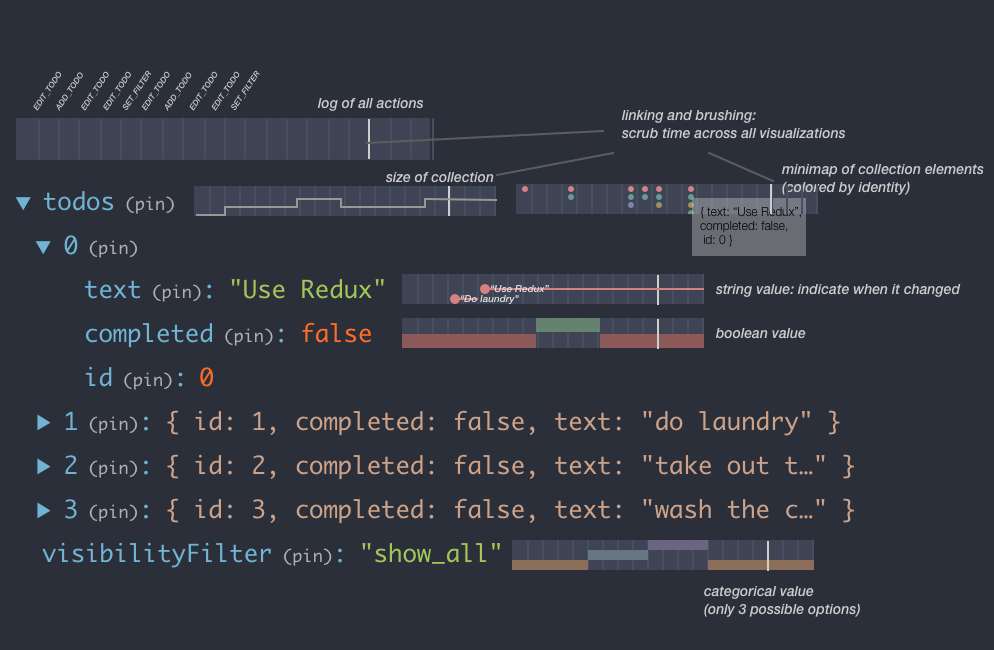
\includegraphics[width=3.4375in,height=2.25in]{images/mockup.png}
\caption{JSON tree with inline sparklines}\label{fig:mockup}
}
\end{figure}

My initial idea, as shown in Figure~\ref{fig:mockup}, was to show the
current state of the application as a nested JSON tree, and then to show
small sparkline-style visualizations next to nodes of the tree. This
design draws some inspiration from \autocite{hoffswell2018a}, but
differs in that it uses visualization to annotate the application's
state tree, rather than its source code. The advantage of this design is
that it closely and directly links the current state to data from the
execution history, but that link also causes thorny problems---for
example, how do you deal with nodes that have disappeared from the
current state? Perhaps more concerningly, by tying the visualization to
the \emph{concrete} current state, it limits the ability of the
programmer to create a customized abstract view, removed from the
details of the state.

In my next iteration I switched to a different layout, shown in
Figure~\ref{fig:timeline}: a vertically stacked list of small
visualizations of state over time. Each visualization can display an
arbitrary projection of the app's Redux state. Because the graphs are
horizontally aligned, it's easy to see how different aspects of the
app's state have changed in relation to each other. While I haven't
implemented this yet, I imagine that programmers would be able to
dynamically add visualizations to this list, specifying useful
projections of app state, and deciding what type of visualization to use
for each projection.

\begin{figure}
\hypertarget{fig:timeline}{%
\centering
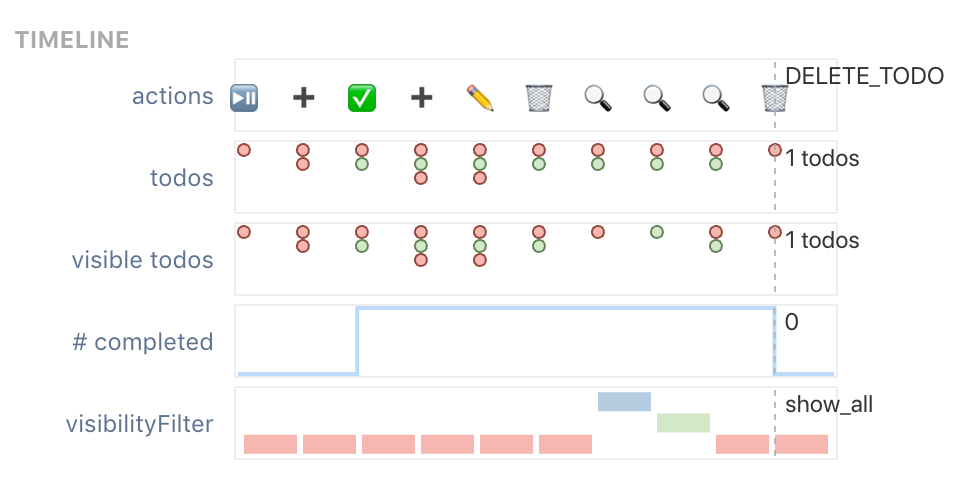
\includegraphics[width=3.4375in,height=1.77083in]{images/timeline.png}
\caption{Timeline view of stacked visualizations}\label{fig:timeline}
}
\end{figure}

One thing lost in the timeline view is the concrete view of the app's
entire state. It's still useful to see this, so I added a separate panel
which displays that data. The user can scrub through history in the
timeline, ``pin'' the app state at a particular point in time, and then
use the separate state view to drill into the app's concrete state at
that point.

\hypertarget{visualization-types}{%
\subsection{Visualization Types}\label{visualization-types}}

Here I describe the specific visualizations I prototyped for the
timeline view. These are shown in Figure~\ref{fig:timeline} from top to
bottom. (The video demo linked on the project page might be an easier
way to grasp the basics of each of these views)

\emph{Action list}: I found that skimming a list of actions represented
as text (\texttt{ADD\_TODO}, \texttt{EDIT\_TODO}, etc.) required a lot
of conscious reading effort. Instead, by choosing a colorful symbol for
each action in the app, we can take advantage of pre-attentive
processing to more quickly understand what actions have occurred in the
execution trace. In this case I chose symbols for all the actions in
TodoMVC; more generally, a programmer could specify a meaningful symbol
for every action in their application. In some cases it might be
difficult to choose meaningful and different symbols for all actions;
falling back to random symbols or colored dots could work as well. In
using this tool I've found that the symbolic action list makes it far
easier to find a point in an execution trace that I'm looking for.

\emph{Collection graph}: This visualization represents the contents of a
collection with a series of vertically stacked dots. The size of the
cluster of dots provides a rough sense of collection size, and the
programmer can more carefully examine the view to get an exact count.

Each dot has a color encoding for some attribute of the collection
element; in this case I've chosen to color the dots by whether the todo
is completed or not. Another available option is to color the dots by
identity---each unique element gets its own color.

I originally represented the list of todos with a line graph showing its
length, but this view allows us to display an additional dimension of
information for each todo. One corresponding weakness of this view is
that the size encoding doesn't offer too much information for
pre-attentive processing when there are more than a few elements so the
relative size change is small. It's not immediately obvious where in the
trace the number of todos changed, whereas a line graph makes it more
obvious. (One possible improvement would be to only show the dots on a
time step where the collection was changed.)

\emph{Line graph}: This is simply a line graph of some numeric quantity
over time. In this context I've used it to visualize quantities like
``Number of todos visible''. Choosing a y-axis is quite tricky because
the full range of values can't be known in advance. In trying out
different options and using the tool myself, I decided that viewing
relative changes over time was most important---generally I'm looking
for things like ``when did the number of todos go down?''. Therefore, I
let each graph scale to the current range of values and don't even show
a y-axis label---I'm not aiming to precisely read numeric values off the
graph.

\emph{Enum graph}: User interfaces commonly have enums / union types,
which can take on a small number of predefined values. To represent enum
values changing over time, I chose to use both a color and position
encoding, as a way of redundantly encoding the information and .

With more time, I'd like to explore many other types of visualizations
in addition to these. One particular interest is displaying the entire
state of a collection of objects in a single graph.

\hypertarget{prototype-implementation}{%
\subsection{Prototype Implementation}\label{prototype-implementation}}

I implemented a working prototype on top of the existing Redux Dev
Tools, which provides substantial infrastructure for inspecting and
manipulating the state of a Redux application. My tool is implemented as
a Redux Dev Tools ``monitor'' which can plug in to those existing APIs.

I used the React and Redux frameworks to implement the main skeleton of
my system. The graphs are built in a combination of d3 and React. I use
d3 for computing scales and positions, and then React for actually
rendering out SVGs.

\hypertarget{sec:discussion}{%
\subsection{Discussion and Future Work}\label{sec:discussion}}

This work is still an early prototype and there are many opportunities
for future work.

Using this system myself, I found that I was able to more quickly get an
overall sense of what happened in an execution trace by looking at these
visualizations than looking at the existing Redux Dev Tools display.
However, I want to gain a clearer understanding of what questions people
have when learning about the behavior of a UI, in order to evaluate the
usefulness of the system. In particular, I'm curious about general
``program understanding'' as opposed to targeted debugging. Could this
visualization be a useful aid when onboarding someone into a codebase
and teaching them how it works?

There's lots of future work to refine the core visualizations further. I
haven't yet explored visualizing a complex object in a single graph, or
showing strings changing over time. I'd also like to more clearly
incorporate Hoffswell et al's taxonomy \autocite{hoffswell2018a} into
this work, evaluating these visualizations in those terms and explicitly
extending that taxonomy.

Another area of work is generalizing this system to work with any Redux
application. I'd like to explore the programmer experience of creating
these visualizations for an existing complex application. How much of
that process can be automated? How can we make it easy for the
programmer to decide which visualizations would be helpful, and then to
actually specify those visualizations? As an initial idea, I imagine
that the programmer could specify an arbitrary expression over the Redux
state,choose from a predefined list of visualizations for showing the
output of that expression, and then add that to the timeline panel in
this tool.

Program visualization offers a rich set of possibilities for helping
people understand their code better. In this work, I've provided an
initial prototype of a system for visualizing the runtime state of
Model-View-Update user interfaces, exploiting the natural architecture
of these applications to show an abstract picture of code execution over
time.

% Balancing columns in a ref list is a bit of a pain because you
% either use a hack like flushend or balance, or manually insert
% a column break.  http://www.tex.ac.uk/cgi-bin/texfaq2html?label=balance
% multicols doesn't work because we're already in two-column mode,
% and flushend isn't awesome, so I choose balance.  See this
% for more info: http://cs.brown.edu/system/software/latex/doc/balance.pdf
%
% Note that in a perfect world balance wants to be in the first
% column of the last page.
%
% If balance doesn't work for you, you can remove that and
% hard-code a column break into the bbl file right before you
% submit:
%
% http://stackoverflow.com/questions/2149854/how-to-manually-equalize-columns-
% in-an-ieee-paper-if-using-bibtex
%
% Or, just remove \balance and give up on balancing the last page.
%
\balance{}

% \bibliographystyle{SIGCHI-Reference-Format}
% \bibliography{sample}

\printbibliography

\end{document}

%%% Local Variables:
%%% mode: latex
%%% TeX-master: t
%%% End:
